\chapter{Future Works and Conclusion}\label{chap:conclusion}
Certain measurable quantities are valued because of the information they reveal about the geometry of the Fermi surface. Additionally, these quantities are attractive because they depend only on universal constants, experimentally controlled variables, and information about the electronic band structure which is entirely determined by the shape of the Fermi surface \cite{Ashcroft_SolidStatePhysics1978}. These measurable quantities commonly arise in the presence of a strong magnetic field and low temperature system. Determining the Fermi surface geometry provides insight into the transport and scattering properties of the material.

\section{Performance Limits in \acp{TMD}}\label{sec:performance_limits}

\section{Integer Quantum Hall Effects}\label{sec:IQHE}
In a \ac{2DES} there are a number of interesting phenomena that occurs at low temperatures in the presence of strong magnetic fields. One such effect is the \ac{IQHE}. The \acs{IQHE} was discovered in 1980 by Klitzing \emph{et al.} \cite{Klitzing_PhysRevLett1980}. They showed that under a quantum regime of temperature and magnetic field there is a quantization of the Hall resistance, which deviates from its linearity in the magnetic field seen in the classical Hall effect, displaying plateaus at particular values of the magnetic field where the Hall resistance is given purely in terms of universal constants. In addition, the plateaus observed in the Hall resistance are accompanied by a vanishing longitudinal resistance \cite{Klitzing_PhysRevLett1980,Ando_RevModPhys1982,Goerbig_2009,Hook_Solid1991}.

\subsection{Theoretical Background}\label{subsec:IQHE_theory}
In order to fully mathematically describe the theory behind the \acs{IQHE} one must first introduce the concept of Landau levels. Here we assume a quantum regime in which there is a low temperature and high magnetic field such that $\hbar\omega\gg k_B T$. The Hamiltonian of a particle in a uniform magnetic field is given by 
\begin{equation}\label{eq:particle_in_b_field}
\hat{H} = \frac{1}{2m}\left(\hat{p}_x+eBy/c\right)^2 + \frac{\hat{p}_y^2}{2m} + \frac{\hat{p}_z}{2m} - \left(\mu/s\right)\hat{s}_z B,
\end{equation}
where $\hat{p}_i$ is the momentum operator in the specified coordinate direction, $B$ is the magnetic field, $e$ is the charge of an electron, $\left(\mu/s\right)\hat{s}_z$ is the intrinsic magnetic moment operator \cite{Landau_Quantum1965}. It is worth noting that the vector potential chosen in eq.~\ref{eq:particle_in_b_field} is known as the Landau gauge, $\vec{A} = \left(-By, 0, 0\right)$, which implies the magnetic field $B$ is directed in the positive $z$-direction \cite{Sakurai_Quantum1994,Landau_Diagmagnetismus1930}. In this case the eigenfunctions of the Hamiltonian must take the form,
\begin{equation}\label{eq:psi_b_field}
\psi\left(\vec{r}\right) = e^{\left(i/\hbar\right)\left(p_x x+p_z z\right)}\chi\left(y\right),
\end{equation} 
where $\chi\left(y\right)$ is defined by solutions to  
\begin{equation}\label{eq:b_field_schrodinger}
	\frac{\partial^2 \chi}{\partial y^2} + \frac{2m}{\hbar^2}\left[E +\left(\mu/s\right)\sigma B - \frac{p_z^2}{2m}-\frac{1}{2}m\left(\frac{e B}{mc}\right)^2\left(y-y_0\right)^2\right]\chi = 0,
\end{equation}
where $y_0 =-c p_x/e B$ and $\omega = \abs{e}B/m c$. Additionally, since the Hamiltonian does not explicitly depend on $x$ and $z$ this implies that both the $x$ and $z$ components of the generalized momentum are conserved. Eq.~\ref{eq:b_field_schrodinger} is formally identical to that of the linear oscillator, thus the expression for the energy levels of a particle in a uniform magnetic field is 
\begin{equation}\label{eq:landau_levels_3D}
	E = \left(n+\frac{1}{2}\right)\frac{\abs{e}\hbar B}{mc} + \frac{p_z^2}{2m} - \left(\mu/s\right)\sigma B,
\end{equation}
where $n$ is any integer \cite{Landau_Quantum1965}. These quantum numbers $n$ specify states known as Landau levels. For the case in which the motion of particles in restricted to a rectangular geometry of $L_x \times L_y$, also let $p_z=0$ as the motion of particles is restricted in this case to only the $x-y$ plane. In this case the energy of each Landau level is given by 
\begin{equation}\label{eq:landau_levels_2D}
	E = \left(n+\frac{1}{2}\right)\frac{\abs{e}\hbar B}{mc} - \left(\mu/s\right)\sigma B.
\end{equation}
Due to the restriction that $\hbar\omega \gg k_B T$, thermal excitations can be neglected because the interval between Landau levels is much greater than thermal excitation energy. As a result, the probability that electrons will be thermally excited to higher energy levels can be neglected. In order to fill higher energy levels the density of states must be increased. When the Landau level is fully occupied from the lowest to the $i\mathrm{th}$ energy level the transverse resistivity becomes
\begin{equation}\label{eq:rho_xy}
	\rho_{xy} = \frac{h}{i e^2},
\end{equation}
where $i$ is any integer corresponding to a specific filled Landau level, $e$ is the charge of an electron, and $h$ is Planck`s constant \cite{Klitzing_PhysRevLett1980,Goerbig_2009}. Eq.~\ref{eq:rho_xy} shows that at critical values of the field, the Hall resistivity (or conductivity) is quantized in units of $h/e^2$ \cite{Kittel_IntroSolidState2005,Hook_Solid1991}. 
\begin{figure}[ht]
	\centering
	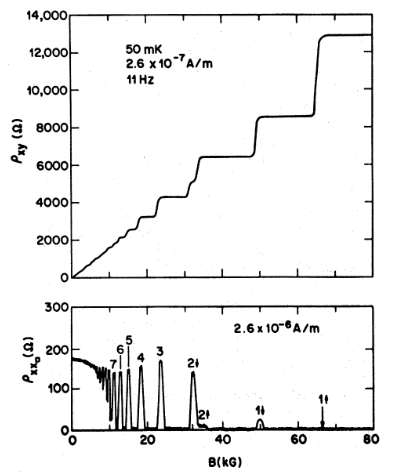
\includegraphics[height=5cm,width=5cm]{figs/future/IQHE_data_RHOxy_RHOxx}
	\caption[Example data of the Integer Quantum Hall Effect]{$\rho_{xy}$ as a function of magnetic field $B$ at low temperature ($T=50\unita{mK}$). Figure originally appeared in ref.~\cite{Paalanen_PhysRevB1982}.}
	\label{fig:IQHE_data}
\end{figure}
Fig.~\ref{fig:IQHE_data} demonstrates an example of the quantized nature of the transverse resistivity. The distance between each plateau (step height) is given by $h/e^2$ divided by an integer $i$. These steplike increases with plateaus in the magnetic field region where the longitudinal resistivity $\rho_{xx}$ vanished \cite{Klitzing_RevModPhys1986}. Thus, when $\rho_{xx} = 0$ then $\rho_{xy} = h/i e^2$ and is at a plateau. Note that the temperatures needed to observe the \acs{IQHE} ($\lesssim 4\unita{K}$) is a likely reason why it was not discovered until 1980. It is also important to note that the value of resistivity only depends on fundamental constants of physics and can be used as a primary resistance standard known as the von Klitzing constant, $R_{\mathrm{K}-90} = 25812.807\unita{\Omega}$ \cite{Klitzing_PhysRevLett1980,Aoki_PhysRevLett1986,Bliek_Met1988}.

\subsection{Implementation and Measuring the Integer Quantum Hall Effect}\label{subsec:IQHE_measure}

\section{Shubnikov-de Haas Oscillations}\label{sec:qm_oscillations}
There are several techniques and measurements that can determine the geometry of the Fermi surface, many of these are closely related to one another and are based on the same underlying mechanism. One such effect is the \acs{SdH} effect \cite{Shubnikov_Leiden1930}. The \acs{SdH} effect is an oscillatory dependence of the resistivity on the magnetic field, there it is related to the \ac{QHE} \cite{Soule_PhysRev1964}. This effect is produced by the oscillation of the density of states at the Fermi level which is caused by the quantization of electron energy levels in the presence of a magnetic field (see sec.~\ref{subsec:IQHE_theory}, Landau levels) \cite{Peierls_ZPhys1933,Landau_RoyalSoc1939}. 

\section{Limitations}\label{sec:limitations}